\documentclass[12pt]{article}
%% arXiv paper template by Flip Tanedo
%% last updated: Dec 2016



%%%%%%%%%%%%%%%%%%%%%%%%%%%%%
%%%  THE USUAL PACKAGES  %%%%
%%%%%%%%%%%%%%%%%%%%%%%%%%%%%

\usepackage{amsmath}
\usepackage{amssymb}
\usepackage{amsfonts}
\usepackage{graphicx}
\usepackage{xcolor}
\usepackage{nopageno}
\usepackage{enumerate}
\usepackage{parskip}
\usepackage{bbm}

\usepackage{sectsty}
\sectionfont{\Large}
% \subsectionfont{\large}
% \renewcommand{\thesection}{}
% \renewcommand{\thesubsection}{\arabic{subsection}}

%%%%%%%%%%%%%%%%%%%%%%%%%%%%%%%%%%%%%%%%%%%%%%%
%%%  PAGE FORMATTING and (RE)NEW COMMANDS  %%%%
%%%%%%%%%%%%%%%%%%%%%%%%%%%%%%%%%%%%%%%%%%%%%%%

\usepackage[margin=2cm]{geometry}   % reasonable margins

\graphicspath{{figures/}}	        % set directory for figures

% for capitalized things
\newcommand{\acro}[1]{\textsc{\MakeLowercase{#1}}}    

\numberwithin{equation}{section}    % set equation numbering
\renewcommand{\tilde}{\widetilde}   % tilde over characters
\renewcommand{\vec}[1]{\mathbf{#1}} % vectors are boldface

\newcommand{\dbar}{d\mkern-6mu\mathchar'26}    % for d/2pi
\newcommand{\ket}[1]{\left|#1\right\rangle}    % <#1|
\newcommand{\bra}[1]{\left\langle#1\right|}    % |#1>
\newcommand{\Xmark}{\text{\sffamily X}}        % cross out

\let\olditemize\itemize
\renewcommand{\itemize}{
  \olditemize
  \setlength{\itemsep}{1pt}
  \setlength{\parskip}{0pt}
  \setlength{\parsep}{0pt}
}


% Commands for temporary comments
\newcommand{\comment}[2]{\textcolor{red}{[\textbf{#1} #2]}}
\newcommand{\flip}[1]{{\color{red} [\textbf{Flip}: {#1}]}}
\newcommand{\email}[1]{\texttt{\href{mailto:#1}{#1}}}

\newenvironment{institutions}[1][2em]{\begin{list}{}{\setlength\leftmargin{#1}\setlength\rightmargin{#1}}\item[]}{\end{list}}


\usepackage{fancyhdr}		% to put preprint number



% Commands for listings package
%\usepackage{listings}      % \begin{lstlisting}, for code
%
% \lstset{basicstyle=\ttfamily\footnotesize,breaklines=true}
%    sets style to small true-type



%%%%%%%%%%%%%%%%%%%
%%%  HYPERREF  %%%%
%%%%%%%%%%%%%%%%%%%

%% This package has to be at the end; can lead to conflicts
\usepackage{microtype}
\usepackage[
	colorlinks=true,
	citecolor=black,
	linkcolor=black,
	urlcolor=green!50!black,
	hypertexnames=false]{hyperref}





\begin{document}


\begin{center}

    {\Large \textsc{Short HW 9}:
    \textbf{Loop Diagrams and Renormalizability}}
    
\end{center}

\vskip .4cm

\noindent
\begin{tabular*}{\textwidth}{rl}
	\textsc{Course:}& Physics 165, \emph{Introduction to Particle Physics} (2022)
	\\
	\textsc{Instructor:}& Prof. Flip Tanedo (\email{flip.tanedo@ucr.edu})
	\\
	\textsc{Due by:}& \textbf{Thursday}, May 26
\end{tabular*}

\section{Vacuum Polarization}

\begin{figure}[h]
	\centering
	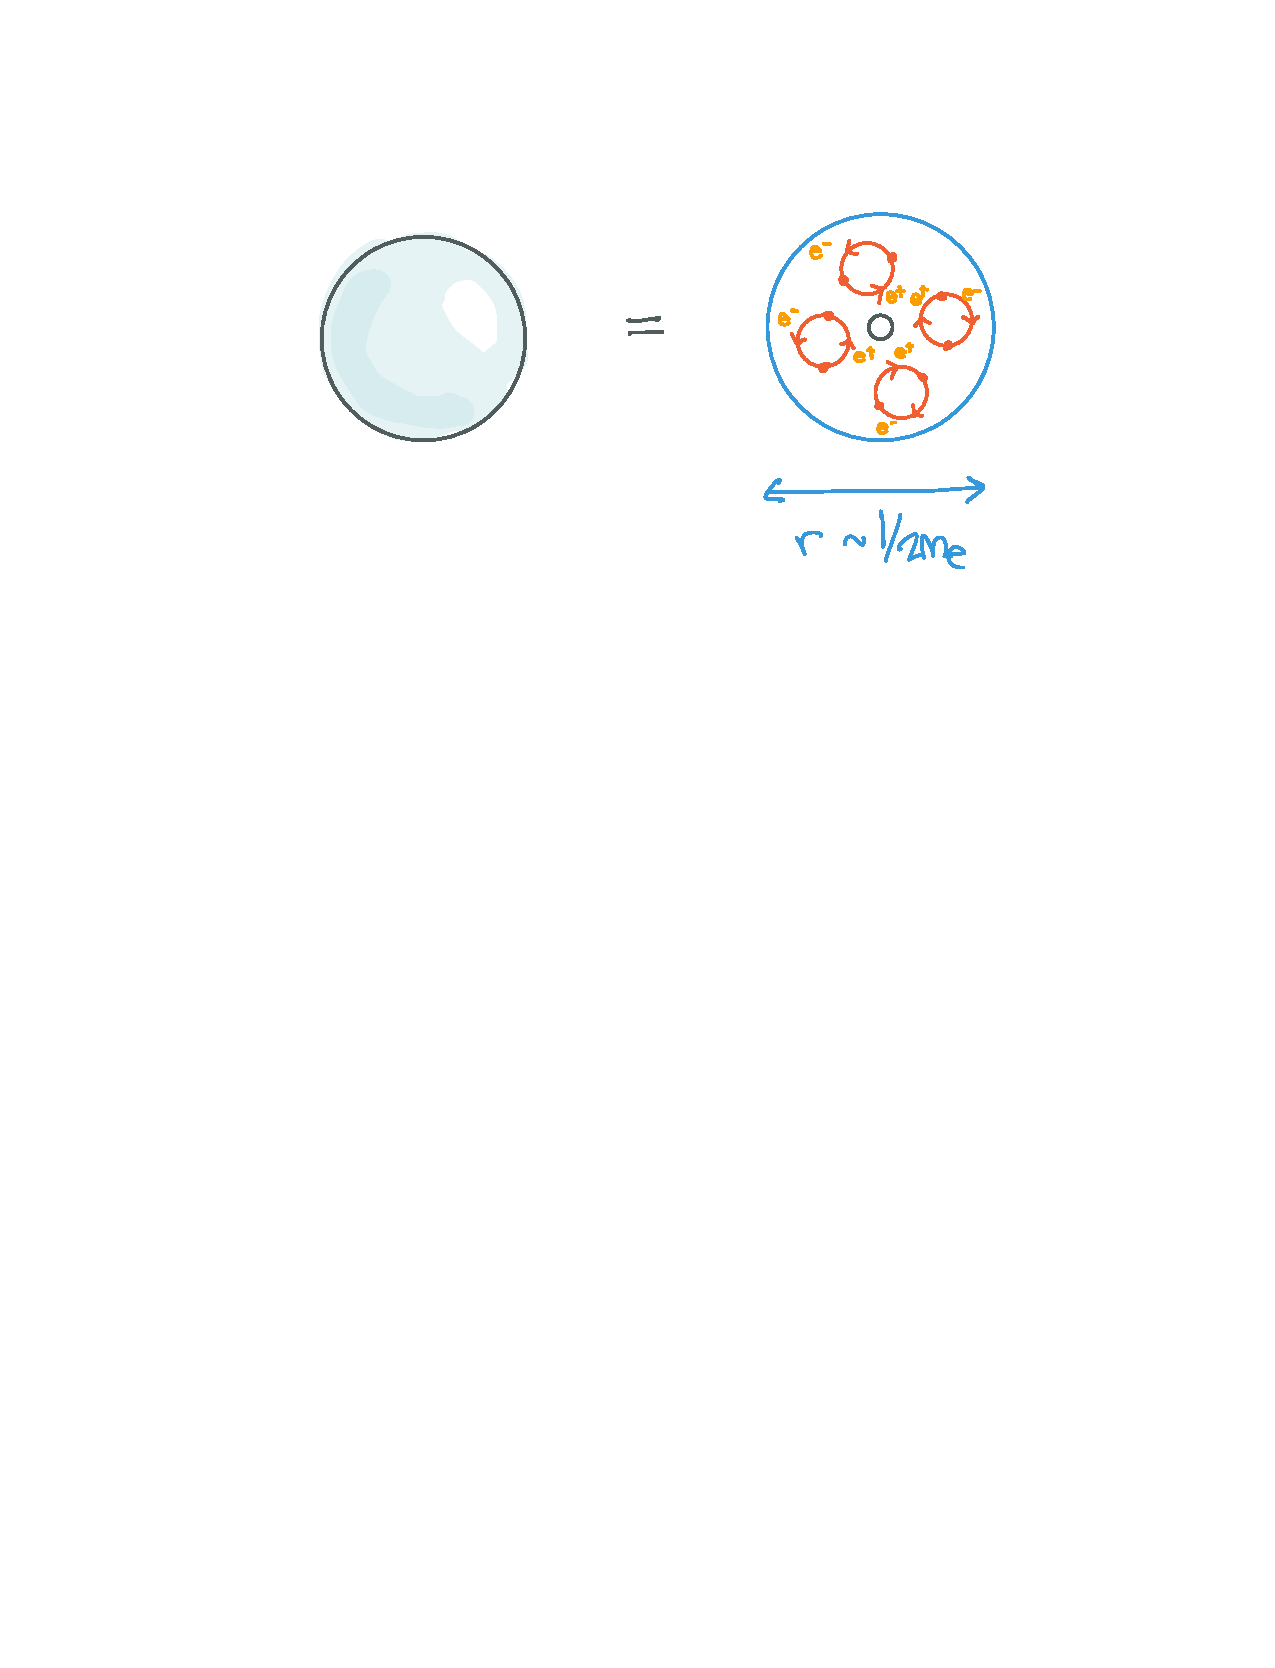
\includegraphics[width=.5\textwidth]{figures/HW9_electron.pdf}
	% \caption{Caption here}
	% \label{fig:figure1}
\end{figure}

On length scales smaller than $L \sim (2m_e)^{-1}$, the production of \emph{virtual} $e^+e^-$ pairs ends up polarizing the vacuum around a charge. This ends up screening a charge and reducing the effective potential at short distances. The effective (observed) mass of the electron is then
\begin{align}
	m_e^{(\text{observed})} = m_e^{(\text{bare})}  + \Delta E \ ,
\end{align}
where $\Delta E \approx \alpha (2m_e)^{-1}$ and $\alpha = e^2/4\pi \approx 1/137$. The bare electron mass is simply some number in the Lagrangian, but it is never directly observed. Given that $m_e = 0.5$~MeV, show that $\Delta E$ is a small correction compared to the observed value of the electron mass. 

\textsc{Comment}: Compare this to the case where we imagined the electron to be a charged shell of some radius $r_e$ that we wanted to take to zero. In that case, $\Delta E$ from the electrostatic self-repulsion of the shell was much larger than the observed electron mass. That is what is called a hierarchy (or tuning) problem: why is the mass of the electron so much smaller than the energy scale of the quantum corrections? In this example, we show that quantum mechanics saves the day\footnote{One can calculate this correction more explicitly in an honest quantum field theory course.} and that $m_e^{(\text{observed})} \approx m_e^{(\text{bare})}$. 


\section{Non-Renormalizable Self-Interacting Particle}

Consider bosonic particle $\varphi$. Suppose the Lagrangian for $\varphi$ contains a $\varphi^6$ interaction. We argued that this means that the theory is non-renormalizable: the theory necessarily has an infinite number of terms in the Lagrangian whose coefficients are not predicted. These terms are necessary to soak up the divergences in loop diagrams when summing over the allowed loop momenta. 
 

\subsection{Divergent Octopus}

Draw a one-loop diagram with eight external $\varphi$ lines that is logarithmically divergent in the momentum cutoff. Recall that each internal line with loop momentum $k$ goes like $\sim 1/k^2$ at large $k$ and that the loop integral is $d^4k$. 

Now draw another such diagram. There are a bunch of them. Think about an octopus that gets its legs tangled up.

\textsc{Comment:} Given that there is a divergent diagram with eight external legs, we now know that there must also be a $\varphi^8$ term in the Lagrangian whose \emph{bare} coupling is not predicted because it has to soak up the divergence from the octopus diagram.

\subsection{Divergent Duodecapod/dodecapod}

Duodec- is the Latin prefix for 12. Dodeca- is the Greek version. Now that we know that there is a $\varphi^8$ vertex in the theory, draw a diagram that has twelve external lines. 

\textsc{Comment:} now we know that there should also be a $\varphi^{12}$ vertex in the theory whose \emph{bare} coupling is not predicted because it has to soak up the dodecapod divergence. You see how this gets problematic, yes? We end up with an infinite number of terms in the Lagrangian, each with an undetermined bare coupling that has to be fixed. 

\textsc{Comment:} The real significance is that each one of these $n$-point interactions has to be physically measured to determine anything about the theory. As a theorist, I do not think I could do one experiment... let alone an infinite number of them. 

\subsection{Is this diagram divergent?}

Here's a diagram of the scalar field $\varphi$ that contributes to the scattering of eight $\varphi$ particles. 
\begin{figure}[h]
	\centering
	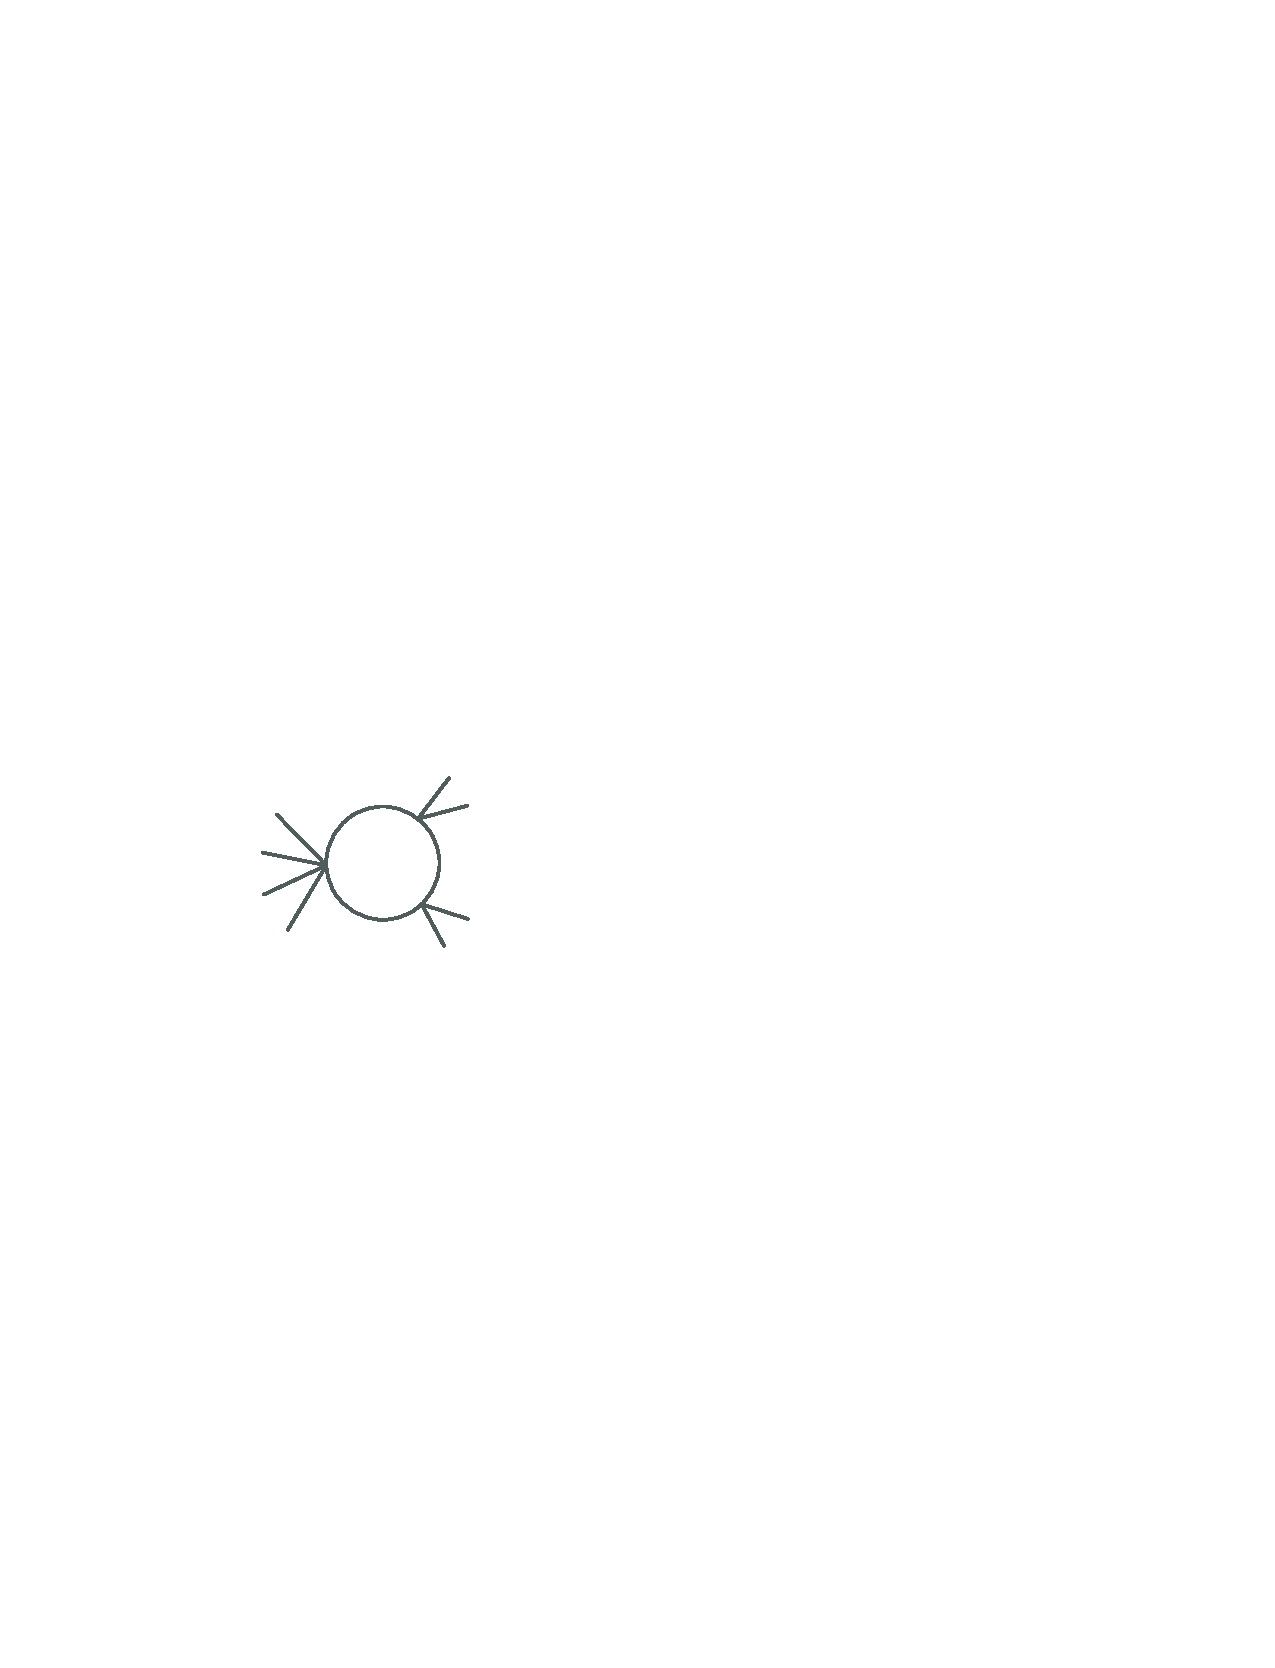
\includegraphics[width=.3\textwidth]{figures/hw9_8pt.pdf}
	% \caption{Caption here}
	% \label{fig:figure1}
\end{figure}
Is this diagram divergent for large loop momentum, $k$? Do the power counting to explain why or why not.



\end{document}